% Présentation de 5 minutes : une baseline commune, trois leviers, leur comparaison. Une idée et une preuve par slide.
%
% Figures :   python slides/make_comparison_figures.py --weights <dossier> (depuis la racine du repo)
% Compiler :  pdflatex comparaison.tex (deux fois, depuis ce dossier)
\documentclass[aspectratio=169,12pt]{beamer}
\usepackage[utf8]{inputenc}
\usepackage[T1]{fontenc}
\usepackage{lmodern}
\usepackage[french]{babel}
\usepackage{amsmath,booktabs}
\graphicspath{{figures/}{../figures/baseline/}{../figures/inference/}}

\definecolor{ink}{HTML}{0B0B0B}
\definecolor{muted}{HTML}{52514E}
\definecolor{warm}{HTML}{EB6834}
\definecolor{surface}{HTML}{FCFCFB}
\setbeamercolor{background canvas}{bg=surface}
\setbeamercolor{normal text}{fg=ink}
\setbeamercolor{frametitle}{fg=ink}
\setbeamercolor{title}{fg=ink}
\setbeamercolor{author}{fg=muted}
\setbeamerfont{frametitle}{size=\large,series=\bfseries}
\setbeamerfont{title}{size=\LARGE,series=\bfseries}
\setbeamertemplate{navigation symbols}{}
\setbeamertemplate{footline}{\hfill{\scriptsize\color{muted}\insertframenumber}\hspace{1em}\vspace{0.5em}}

% Protocole de la mesure, en bas de slide.
\newcommand{\source}[1]{\vfill{\scriptsize\color{muted}#1\par}}
% Figure du fichier #1, ou mention d'attente tant que la mesure n'est pas terminée.
\newcommand{\mesure}[2]{\IfFileExists{figures/#1}{\includegraphics[#2]{#1}}{\vspace{3em}{\color{warm}\textbf{À compléter :} mesure en cours}}}

\title{À générateur imposé, que peut-on gagner ?}
\author{Quentin Revillon, Noé Mosca, Nicodème Gorge\\[0.3em]Groupe 3}
\date{}

\begin{document}

\begin{frame}[plain,noframenumbering]
  \titlepage
\end{frame}

\begin{frame}{Le générateur est imposé : trois leviers restent}
  \centering\vspace{1.2em}
  {\large $z \in \mathbb{R}^{100} \;\longrightarrow\; G \;\longrightarrow\; x \in [-1,1]^{784}$}\\[0.3em]
  {\small\color{muted} MLP imposé : $100 \to 256 \to 512 \to 1024 \to 784$}

  \vspace{1.6em}
  {\small\begin{tabular}{lll}
    \toprule
    Levier & Question & Méthodes \\
    \midrule
    \textbf{Données} & que voit le GAN ? & sélection, bruit d'instance \\
    \textbf{Entraînement} & comment apprend-il ? & perte R3GAN \\
    \textbf{Inférence} & comment tirer les images ? & Discriminator Rejection Sampling \\
    \bottomrule
  \end{tabular}}

  \vspace{1.6em}
  {\large Qu'améliore chaque levier : la \textbf{qualité} ou la \textbf{diversité} ?}
\end{frame}

\begin{frame}{Une baseline commune, une seule mesure}
  \vspace{0.6em}
  \begin{columns}[T,onlytextwidth]
    \column{0.42\textwidth}
    \textbf{Baseline}\\[0.5em]
    \small
    Code fourni : perte BCE, Adam, lr $2\cdot10^{-4}$\\[0.3em]
    Batch 100, 200 époques\\[1em]
    \textbf{Split}\\[0.5em]
    \begin{tabular}{@{}ll@{}}
      train & 50\,000 : entraîner \\
      val & 10\,000 : choisir \\
      test & 10\,000 : chiffres finaux \\
    \end{tabular}
    \column{0.54\textwidth}
    \textbf{FID} (Inception)\\[0.3em]
    {\small $\|\mu_r-\mu_g\|^2 + \mathrm{Tr}\big(\Sigma_r+\Sigma_g-2(\Sigma_r\Sigma_g)^{1/2}\big)$}\\[1em]
    \textbf{Précision} (VGG, $k=5$) : qualité\\[0.3em]
    {\small part des images générées dans la zone des vraies}\\[1em]
    \textbf{Rappel} (VGG, $k=5$) : diversité\\[0.3em]
    {\small part des vraies images dans la zone des générées}
  \end{columns}
  \source{{\color{warm}À retirer après le réentraînement :} baseline et inférence suivent ce split ; données et entraînement sont en cours de réentraînement dessus.}
\end{frame}

\begin{frame}{Baseline : 200 époques, et deux mesures qui se contredisent}
  \centering\vspace{0.3em}
  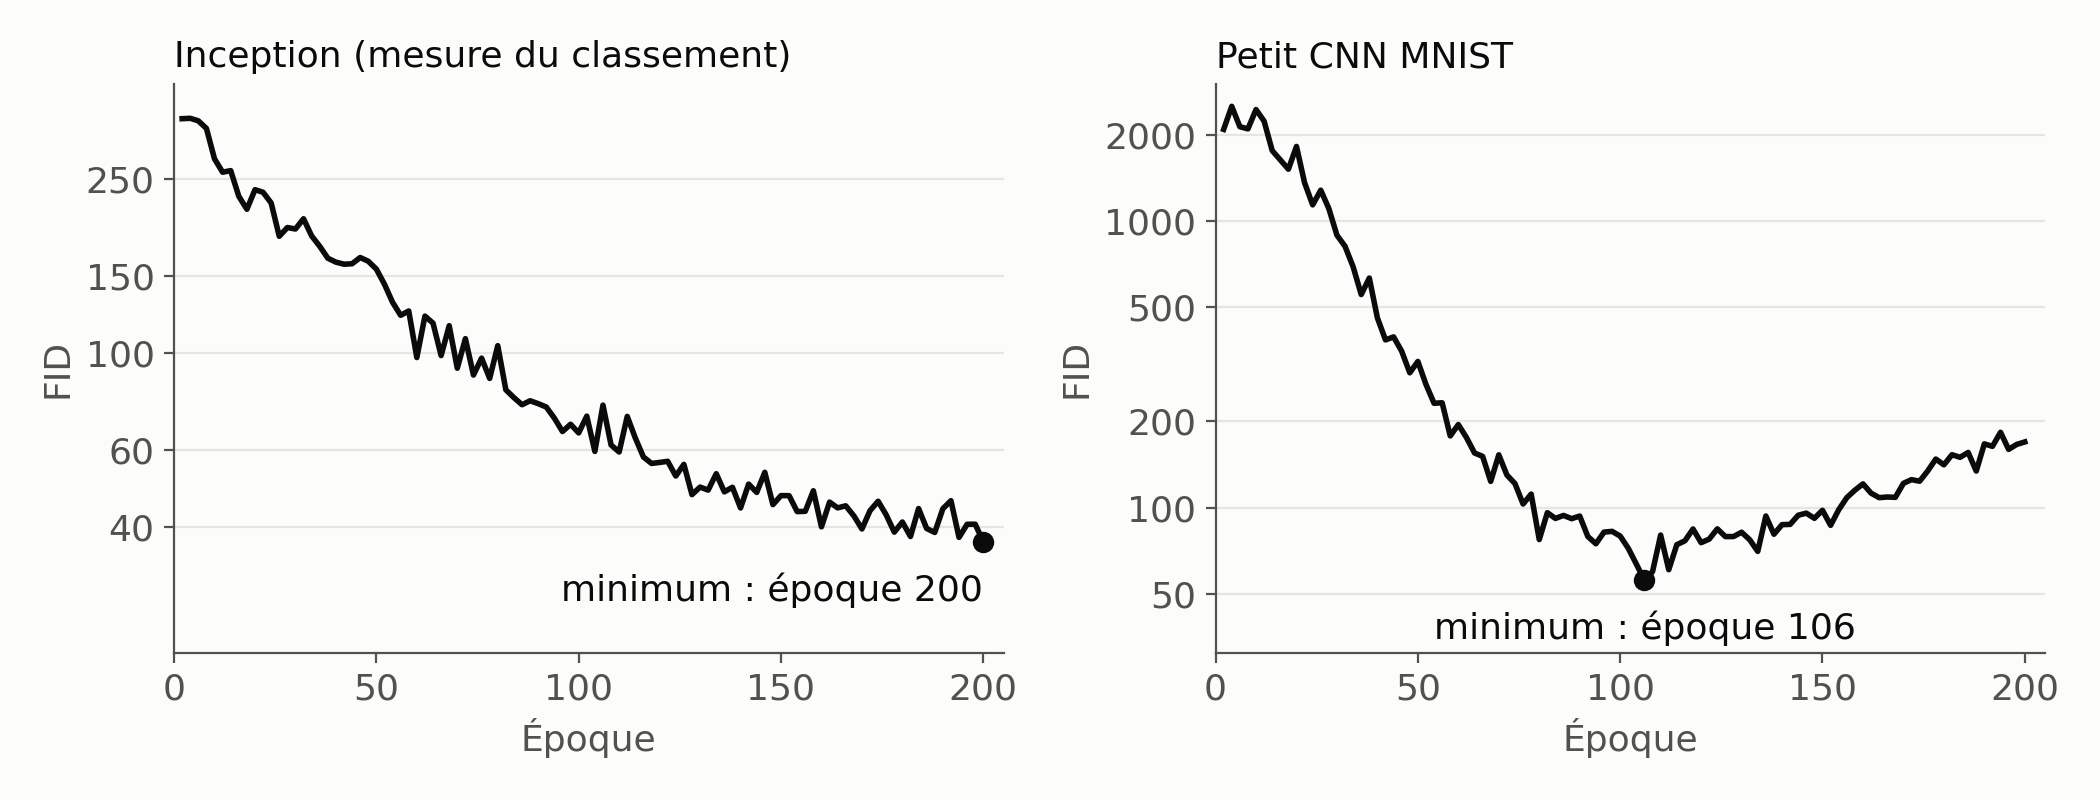
\includegraphics[width=\linewidth]{cmp_two_measures.png}
  \source{Mêmes poids dans les deux panneaux. 10\,000 images contre val, toutes les 2 époques. Deux entraînements complets donnent des poids identiques au bit près.}
\end{frame}

\begin{frame}{Le FID du petit CNN mesure surtout le mélange des chiffres}
  \centering\vspace{0.4em}
  \begin{tabular}{lcc}
    \toprule
    FID du petit CNN & Images telles quelles & Chiffres remis en proportion \\
    \midrule
    Époque 120 & 75,4 & \textbf{30,3} \\
    Époque 200 & 169,4 & \textbf{32,2} \\
    \bottomrule
  \end{tabular}

  \vspace{0.8em}
  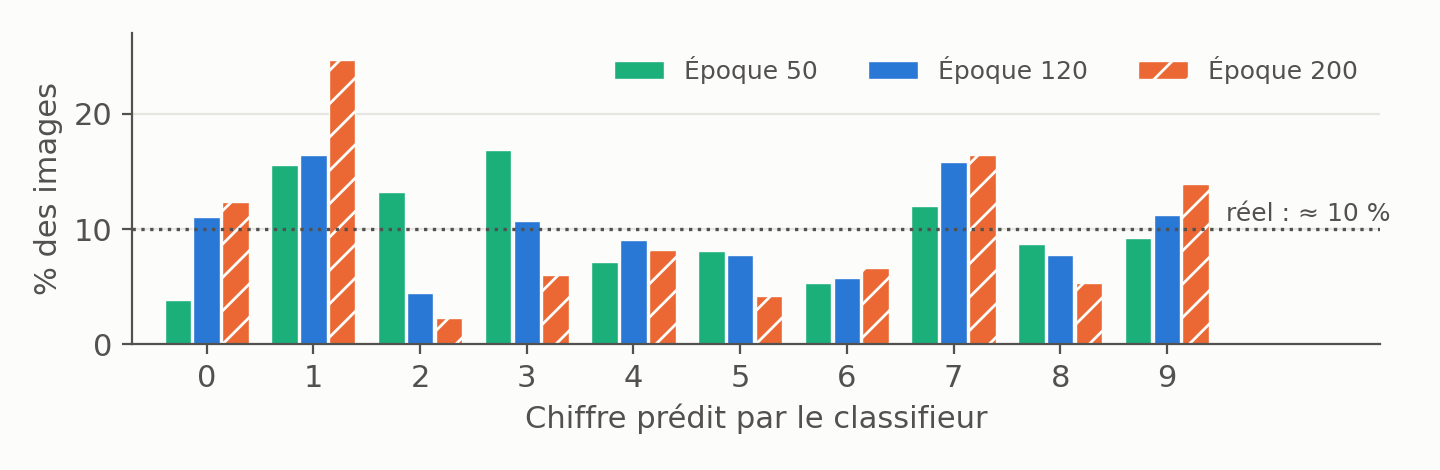
\includegraphics[width=0.8\linewidth]{baseline_classes.png}

  {\small Le défaut de l'époque 200 : 25\,\% de « 1 », 2\,\% de « 2 ». \textbf{On décide donc avec Inception et VGG.}}
\end{frame}

\begin{frame}{Données : la sélection échange de la diversité contre de la qualité}
  \centering\vspace{0.2em}
  {\small Sélection : garder les images les plus denses de chaque chiffre}\\[0.2em]
  {\small $s(x) = -\big(f(x)-\mu_c\big)^\top \Sigma_c^{-1} \big(f(x)-\mu_c\big)$}\\[0.3em]
  {\small Bruit : $D(x + \sigma_t\,\varepsilon)$, avec $\varepsilon \sim \mathcal{N}(0, I)$ et $\sigma_t$ décroissant vers 0}\\[0.6em]
  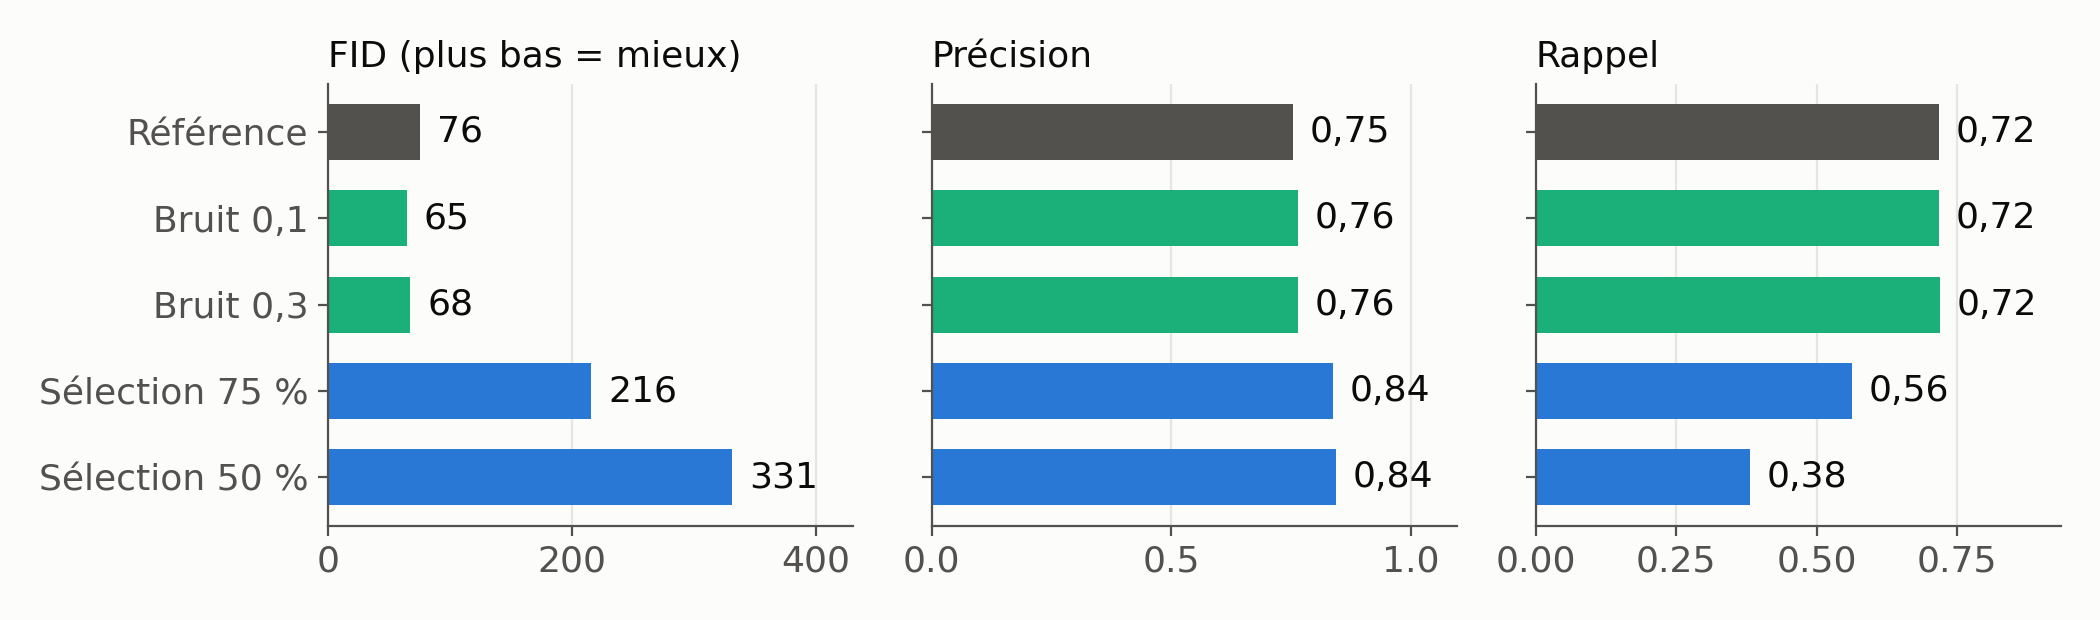
\includegraphics[width=0.92\linewidth]{cmp_data_gain.png}
  \source{DeVries et al. 2020 ; Sønderby et al. 2017. Nicodème : 60\,000 images, 60\,000 mises à jour, petit CNN contre MNIST test, 3 à 8 seeds, runs effondrés exclus (3 sur 8 pour la référence). L'écart du bruit n'est pas significatif (p = 0,10 et 0,23).}
\end{frame}

\begin{frame}{Entraînement : à 50 époques, la perte R3GAN divise le FID par 4}
  \centering\vspace{0.1em}
  {\small $\displaystyle \mathcal{L}_D = \mathrm{softplus}\big(D(G(z)) - D(x)\big) + \frac{\gamma}{2}\big(\underbrace{\|\nabla_x D(x)\|^2}_{R_1} + \underbrace{\|\nabla_x D(G(z))\|^2}_{R_2}\big)$}\\[0.1em]
  {\small $\mathcal{L}_G = \mathrm{softplus}\big(D(x) - D(G(z))\big)$}\\[0.3em]
  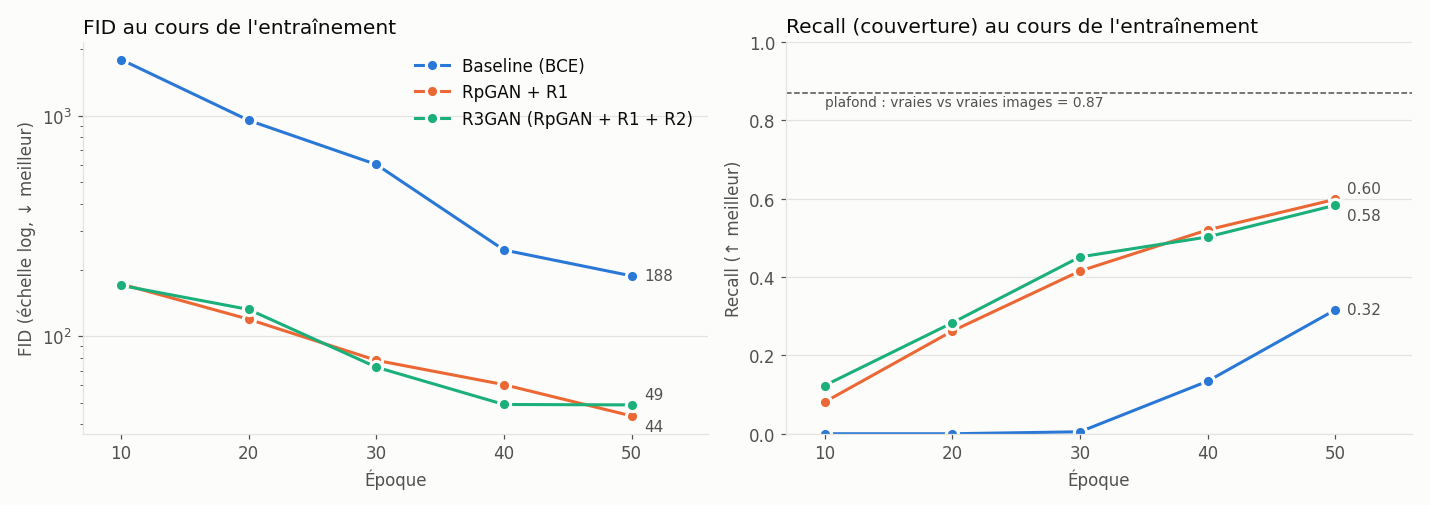
\includegraphics[width=0.78\linewidth]{noe_fid_recall_curves.png}
  \source{Huang et al., NeurIPS 2024 : seule la perte est reprise. Noé : 60\,000 images, 50 époques, petit CNN contre MNIST test, une seed. La baseline n'a pas encore convergé à 50 époques. Sans R1, la perte diverge.}
\end{frame}

\begin{frame}{Inférence : $D$ note chaque image, on en garde une partie}
  \centering\vspace{0.1em}
  {\small $\displaystyle \frac{p_{\mathrm{réel}}(x)}{p_G(x)} = e^{d(x)}
  \qquad p_{\mathrm{garder}}(x) = \sigma\big(\hat F(x)\big)$}\\[0.2em]
  {\small $\hat F(x) = d(x) - d_M - \log\big(1 - e^{d(x) - d_M - \epsilon}\big) - \gamma$}\\[0.2em]
  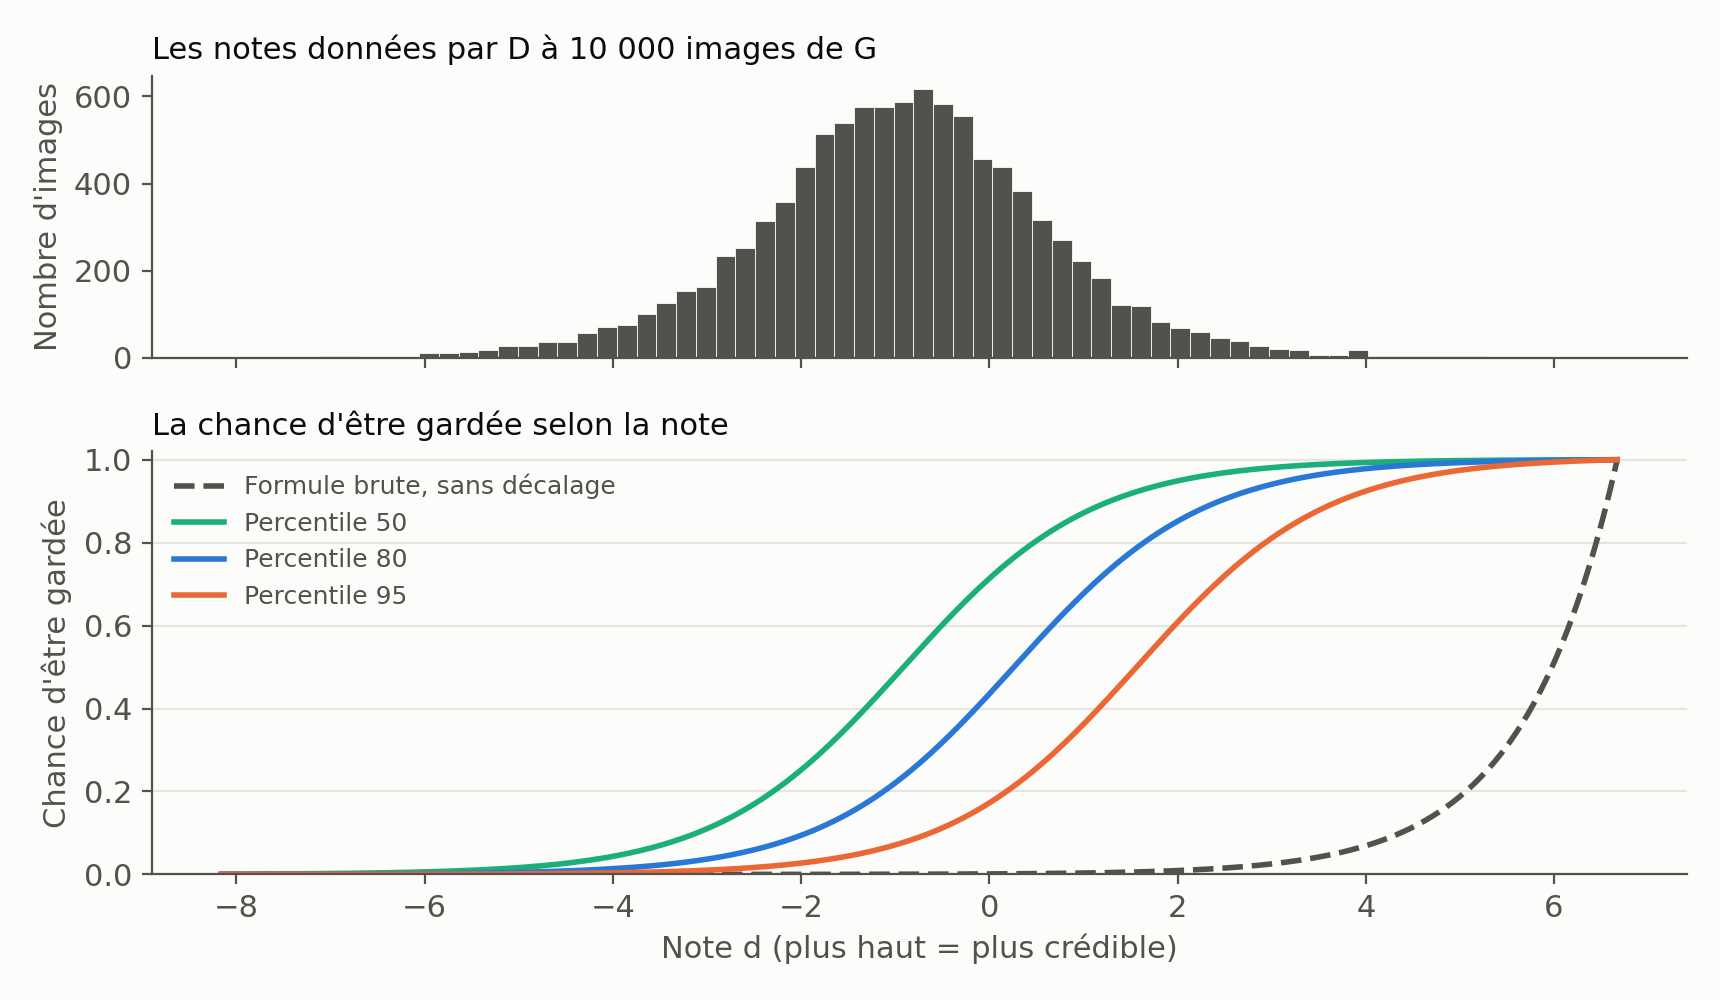
\includegraphics[width=0.56\linewidth]{drs_score_to_chance.png}
  \source{Azadi et al. 2019. $d$ : score de $D$ avant la sigmoïde. $d_M$ : meilleur score observé. $\gamma$ : percentile de $\hat F$ dans chaque batch, qui règle la sévérité du tri. $G$ n'est pas modifié.}
\end{frame}

\begin{frame}{Inférence : un meilleur FID, sans perte de diversité}
  \centering\vspace{0.3em}
  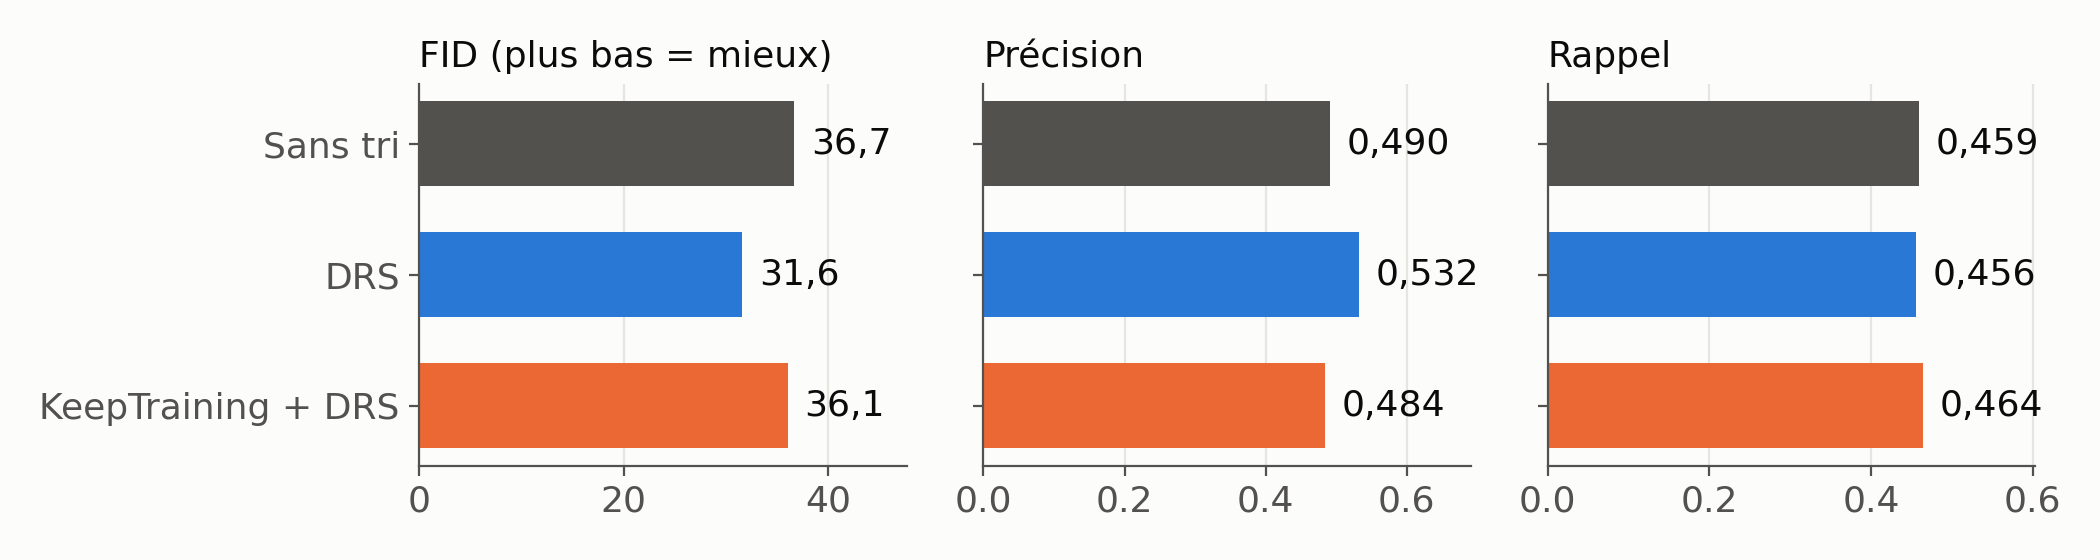
\includegraphics[width=\linewidth]{cmp_drs_gain.png}

  \vspace{0.8em}
  \begin{tabular}{ccc}
    \textbf{30\,\%} & \textbf{1,6 s} & \textbf{31,7} \\
    {\small images gardées} & {\small sur CPU pour 10\,000 images} & {\small FID via \texttt{generate.py}, batch 256}
  \end{tabular}

  \vspace{0.5em}
  {\small L'étape KeepTraining du papier dégrade le FID : on ne la garde pas.}
  \source{Époque 200, percentile 80. Inception et VGG contre val, 3 tirages. Limite de la plateforme : 1\,200 s.}
\end{frame}

\begin{frame}{Comparaison : qui bat la baseline commune ?}
  \centering
  \mesure{cmp_fid.png}{width=\linewidth}
\end{frame}

\begin{frame}{Comparaison : qualité, diversité, équilibre des chiffres}
  \centering\vspace{0.3em}
  \begin{columns}[T,onlytextwidth]
    \column{0.5\textwidth}\centering
    \mesure{cmp_pr.png}{width=\linewidth}
    \column{0.5\textwidth}\centering
    \mesure{cmp_balance.png}{width=\linewidth}
  \end{columns}
\end{frame}

\begin{frame}{Les images}
  \centering\vspace{1.5em}
  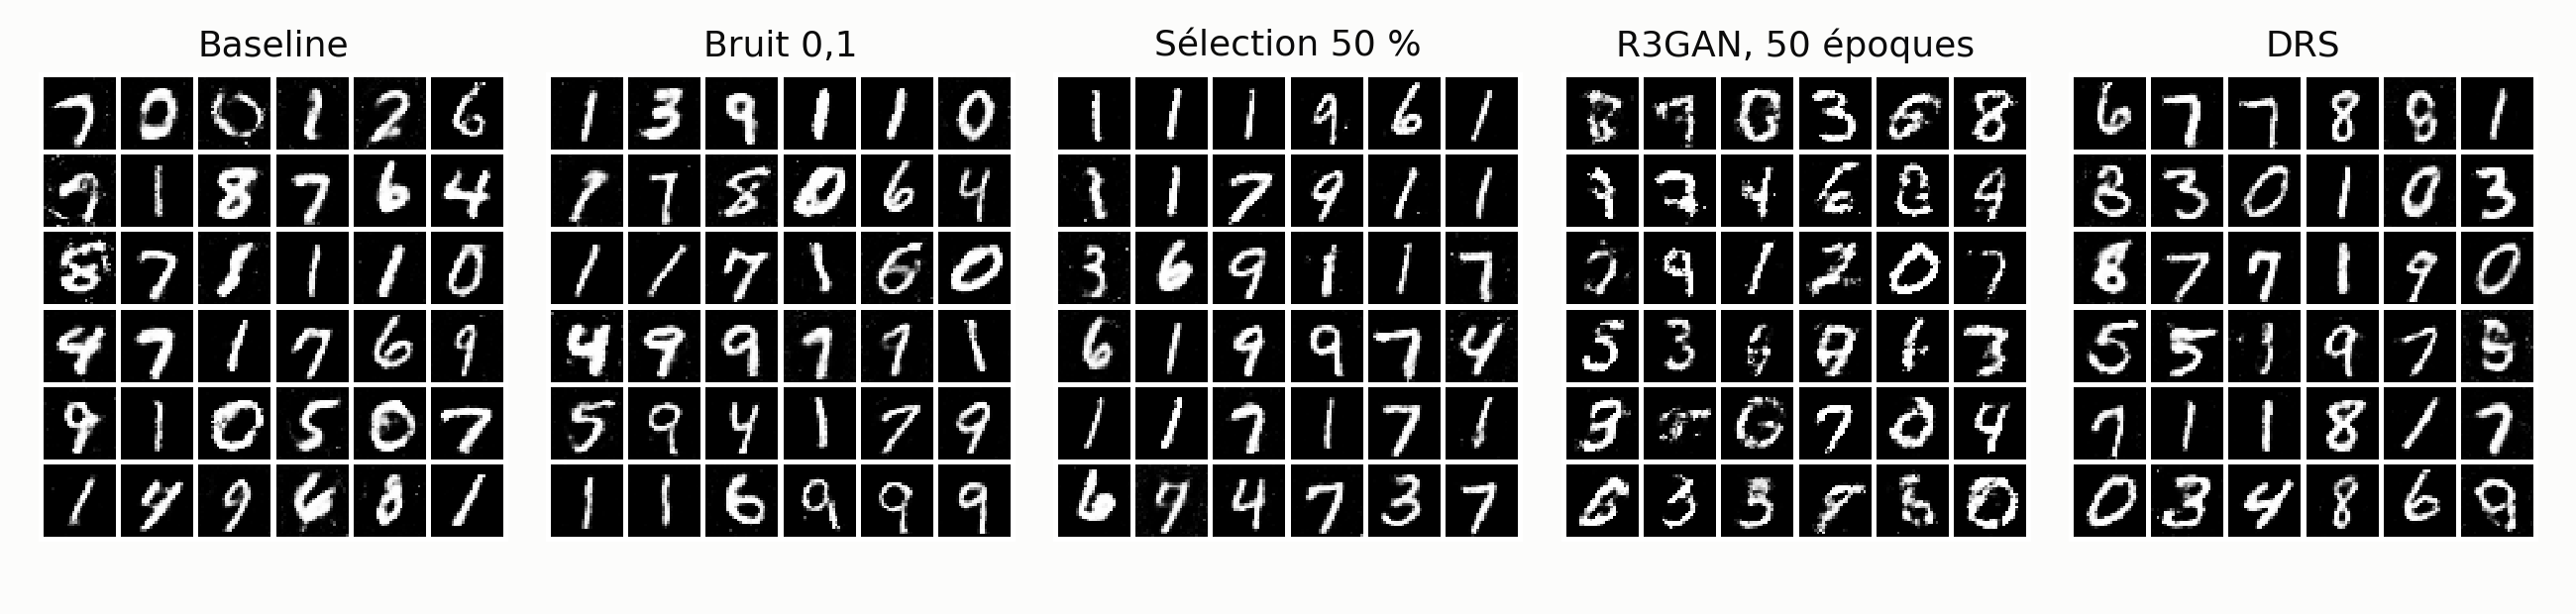
\includegraphics[width=\linewidth]{cmp_samples.png}
  \source{Même bruit dans toutes les grilles, sauf pour le DRS, qui garde une partie des images proposées. R3GAN : 50 époques ; les autres : au moins 200 époques ou un budget équivalent.}
\end{frame}

\begin{frame}{Ce qu'on retient}
  \vspace{1em}
  \begin{itemize}
    \setlength\itemsep{1em}
    \item \textbf{Entraîner plus longtemps :} le FID Inception passe de 156 à 37, mais les chiffres se déséquilibrent.
    \item \textbf{Inférence :} le DRS fait passer le FID de 36,7 à 31,6 pour un coût négligeable, sans corriger l'équilibre.
    \item \textbf{Données :} la sélection échange de la diversité contre de la qualité ; le bruit n'a pas d'effet démontré.
    \item \textbf{Entraînement :} R3GAN accélère fortement l'apprentissage {\color{warm}[à confirmer sur la baseline commune]}.
    \item \textbf{Mesure :} une valeur de FID dépend du réseau utilisé : on ne compare qu'à mesure égale.
  \end{itemize}
\end{frame}

\end{document}
